\documentclass[17pt, t, aspectratio=169, xcolor=table]{beamer}

% To have print without pause
% \documentclass[handout, t, aspectratio=169]{beamer}

\usepackage[utf8]{inputenc}
\usepackage{hyperref}

% Change the presentation layout
\usetheme{Madrid}

% Change the caption size of figure
\usepackage[font=small,skip=4pt]{caption}
\usepackage[symbol]{footmisc}

% Font
\usepackage{plex-sans}

\usepackage[style=numeric,backend=biber,
            doi=false,isbn=false,url=false,eprint=false]{biblatex}
\usepackage{latexsym,xcolor,multicol,booktabs,calligra}
\usepackage{amssymb,amsfonts,amsmath,amsthm,mathrsfs,mathptmx}
\usepackage{graphicx,pstricks,listings,stackengine}
% \usefonttheme[onlymath]{serif}

\usepackage[caption=false]{subfig}
\usepackage{tabularx}
\usepackage{booktabs}

\usepackage{color, colortbl}

% Define color for highlighted table
\definecolor{TableHighLight}{RGB}{190, 250, 196}

\setbeamertemplate{navigation symbols}{}
% \setbeamertemplate{footline}[frame number]
\setbeamertemplate{bibliography item}{\insertbiblabel}
% \setbeamertemplate{footnote}{\insertfootnotetext}

\let\oldfootnotesize\footnotesize
\renewcommand*{\footnotesize}{\oldfootnotesize\tiny}

\DeclareCiteCommand{\footpartcite}[\mkbibfootnote]
{\usebibmacro{prenote}}%
{\usebibmacro{citeindex}%
    \mkbibbrackets{\usebibmacro{cite}}%
    \setunit{\addnbspace}
    \printnames{labelname}%
    \setunit{\labelnamepunct}
    \printfield[citetitle]{title}%
    \newunit
    \printfield[]{year}}
{\addsemicolon\space}
{\usebibmacro{postnote}}

\setbeamertemplate{footnote}{\insertfootnotetext}
\setbeamertemplate{caption}[numbered]

% \usepackage[style=numeric, sorting=none]{biblatex}
 % Insert the structure.tex file which contains the majority of the structure behind the template

%------------------------------------------------------------
%This block of code defines the color theme
\definecolor{ThemeColor}{RGB}{ 40,135, 50} % Elektro- und Informationstechnik
% \definecolor{ThemeColor}{RGB}{ 25,130,130} % Architektur- und Bauwesen
%\definecolor{ThemeColor}{RGB}{ 40,105,175} % Maschinenbau und Mechatronik
%\definecolor{ThemeColor}{RGB}{ 30, 70,150} % Wirtschaftswissenschaften
%\definecolor{ThemeColor}{RGB}{100, 55,140} % Informatik und Wirtschaftsinformatik
%\definecolor{ThemeColor}{RGB}{140, 45,130} %Informationsmanagement und Medien
\usecolortheme[named=ThemeColor]{structure}

%------------------------------------------------------------
%This block of code defines the information to appear in the
%Title page
\title[Short Title] %optional
{Presentation Title}

\subtitle{Sub-title}

\author[Last Name, First name] % (optional)
{Last name, First Name
first.lastname@h-ka.de}

\date[April 27th, 2023] % (optional)
{April 27th, 2023}


%%%% Definition of Layout metrics

\newcommand{\covertextsize}{44}
\newcommand{\titletextsize}{32}
\newcommand{\contenttextsize}{18}

\newcommand{\leftmarginpos}{0.9335cm}

\newcommand{\topmargintitle}{-0.825cm}

\newcommand{\topmargincontent}{3.5cm}

\newcommand{\maximumwidth}{31.9cm}
\newcommand{\maximumheight}{12.6cm}

\newcommand{\columnmaxwidth}{15.45cm}
\newcommand{\secondcolumnstart}{17.38cm}

\newcommand{\captionsize}{large}
\usepackage[font=\captionsize,skip=4pt]{caption}

\definecolor{TableHighLight}{RGB}{190, 250, 196}

%%%%

\addbibresource{bibliography.bib}

%End of title page configuration block
%------------------------------------------------------------

\makeatletter
\def\@makefnmark{}

\begin{document}

\EITCoverVI{Wilkommen}{Vorname Nachname}

\EITTableOfContent{Content}{2}

\section{Normal Content Slide}

\EITHeadlineFT{Normal Content Slide}{
    \lipsum[2]
}

\section{Slide with Columns}
\EITHeadlineFT{Slide with two seperate columns}
{
    \placetextbox{\leftmarginpos}{-\topmargincontent}{\columnmaxwidth}{
        \lipsum[1]
    }
    \placetextbox{\secondcolumnstart}{-\topmargincontent}{\columnmaxwidth}{
        \lipsum[2]
    }
}

\EITHeadlineFT{Slide with Floating Columns}
{
    \placetextbox{\leftmarginpos + 1cm}{-\topmargincontent - 1cm}{\columnmaxwidth}{
        \lipsum[1]
    }
    \placetextbox{\secondcolumnstart}{-\topmargincontent + 0.5cm}{\columnmaxwidth}{
        \lipsum[2]
    }
}

\section{Slide with Table}
\EITHeadlineFT{Slide with Table}{
    \begin{table}
    \begin{center}
    \begin{tabular}{||c | c c | c c c||} 
     \hline
     \# & A & B & C \textsuperscript{\dag} & D \textsuperscript{\S} & E\textsuperscript{\dag\dag} \\ [0.5ex] 
     \hline\hline
     1 & A & B & C & D & E \\ 
     \hline
     2 & A & B & C & D & E \\ 
     \hline
    \rowcolor{TableHighLight}
     5 & A & B & C  & D & E \\
     \hline
         
    \rowcolor{TableHighLight}
     6 & A & B & C & D & E \\ [0.2ex] 
     \hline
    \end{tabular}
    \caption{\label{table:highlight} Table with highlights }
    \end{center}
    \end{table}
}

\EITHeadlineFT{Slide with Floating Table}{
    \placetextbox{0.2\paperwidth}{0}{\maximumwidth}{
        \begin{table}
            \begin{tabular}{||c | c c | c c c||} 
             \hline
             \# & A & B & C \textsuperscript{\dag} & D \textsuperscript{\S} & E\textsuperscript{\dag\dag} \\ [0.5ex] 
             \hline\hline
             1 & A & B & C & D & E \\ 
             \hline
             2 & A & B & C & D & E \\ 
             \hline
            \rowcolor{TableHighLight}
             5 & A & B & C  & D & E \\
             \hline
                 
            \rowcolor{TableHighLight}
             6 & A & B & C & D & E \\ [0.2ex] 
             \hline
            \end{tabular}
            \caption{\label{table:highlight} Table with highlights }
            \end{table}    
    }
}

\section{Slide with Image}
\EITHeadlineFT{Slide with one Image}
{
    \placetextbox{\leftmarginpos}{-\topmargincontent}{\maximumwidth}{
        \picdims[width=\maximumwidth]{\maximumwidth}{\maximumheight}{Pictures/csm_HKA_FK-EIT_2017-9363_a9e6e1d039.jpg}
    }
}


\EITHeadlineFT{Slide with two Images}{
\placetextbox{\leftmarginpos}{-\topmargincontent}{\columnmaxwidth}{
    \picdims[width=\paperwidth]{\columnmaxwidth}{\maximumheight}{Pictures/csm_HKA_FK-EIT_2017-9363_a9e6e1d039.jpg}
}

\placetextbox{\secondcolumnstart}{-\topmargincontent}{\columnmaxwidth}{
    \picdims[width=\paperwidth]{\columnmaxwidth}{\maximumheight}{Pictures/csm_HKA_FK-EIT_2017-9363_a9e6e1d039.jpg}
}
}

\EITHeadlineFT{Slide with Floating Image}
{
    \placetextbox{\leftmarginpos + 0.2\paperwidth}{-\topmargincontent - 5cm}{\maximumwidth}{
        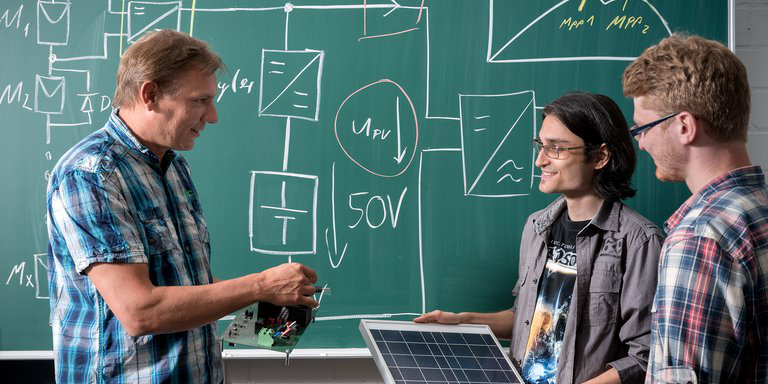
\includegraphics[scale=0.5]{Pictures/csm_HKA_FK-EIT_2017-9363_a9e6e1d039.jpg}
    }
}



\EITHeadlineFT{Slide with Text and Image}{

\placetextbox{\leftmarginpos}{-\topmargincontent}{\columnmaxwidth}{
    \lipsum[2]
}

\placetextbox{\secondcolumnstart}{-\topmargincontent}{\columnmaxwidth}{
    \picdims[width=\paperwidth]{\columnmaxwidth}{\maximumheight}{Pictures/csm_HKA_FK-EIT_2017-9363_a9e6e1d039.jpg}
}
}

\EITHeadlineFT{}{

\placetextbox{0cm}{0cm}{\paperwidth}{
    \picdims[width=\paperwidth]{\paperwidth}{16cm}{Pictures/csm_HKA_FK-EIT_2017-9363_a9e6e1d039.jpg}
}

}

\EITHeadlineFT{References}{

\begin{itemize}
    \item \fullcite{article_key}
    \item \fullcite{book_key}

\end{itemize}


}

\end{document}